\section{Uncertainties}
\label{891_2:sec:uncertainty}

Uncertainties in our derived parameters ($\tau_L$, $Z_L$, $A_V$) come
from a number of sources: the precision and accuracy of the data
(e.g., random errors and flux calibration, respectively); degeneracies
between age, metallicity, and extinction as coupled in the model
parameters; and systematic uncertainty in our interpretation of the
results of the fit. In the context of our DFK basis set, the latter
consists of the assignment of the effective age of each template,
which then propogates into the mass- or light-weighted mean age and
metallicity.  In this section we quantify the magnitude of these
uncertainties, first looking at the coupling between random errors in
the data and covariance in age, metallicity, and extinction.
 

\subsection{Stochastic Uncertainty and Covariance}
\label{891_2:sec:fit_err}

\begin{figure*}
  \centering
  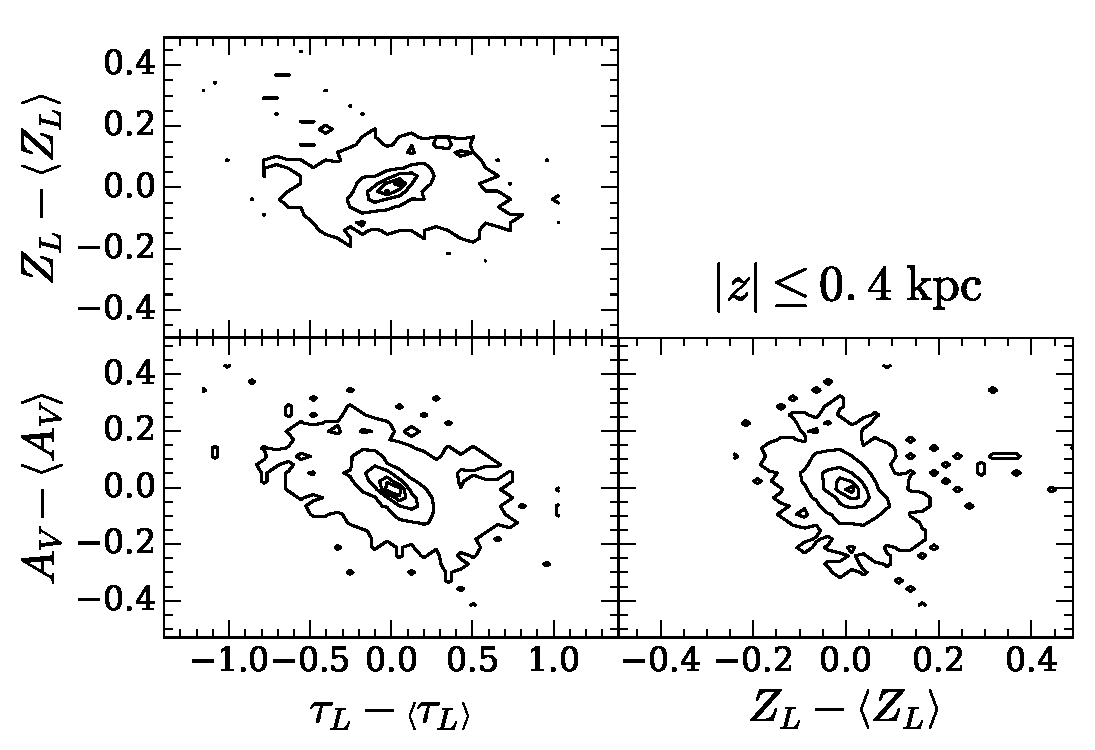
\includegraphics[width=0.48\textwidth]{891_2/figs/MC_covarcont_below.pdf}
  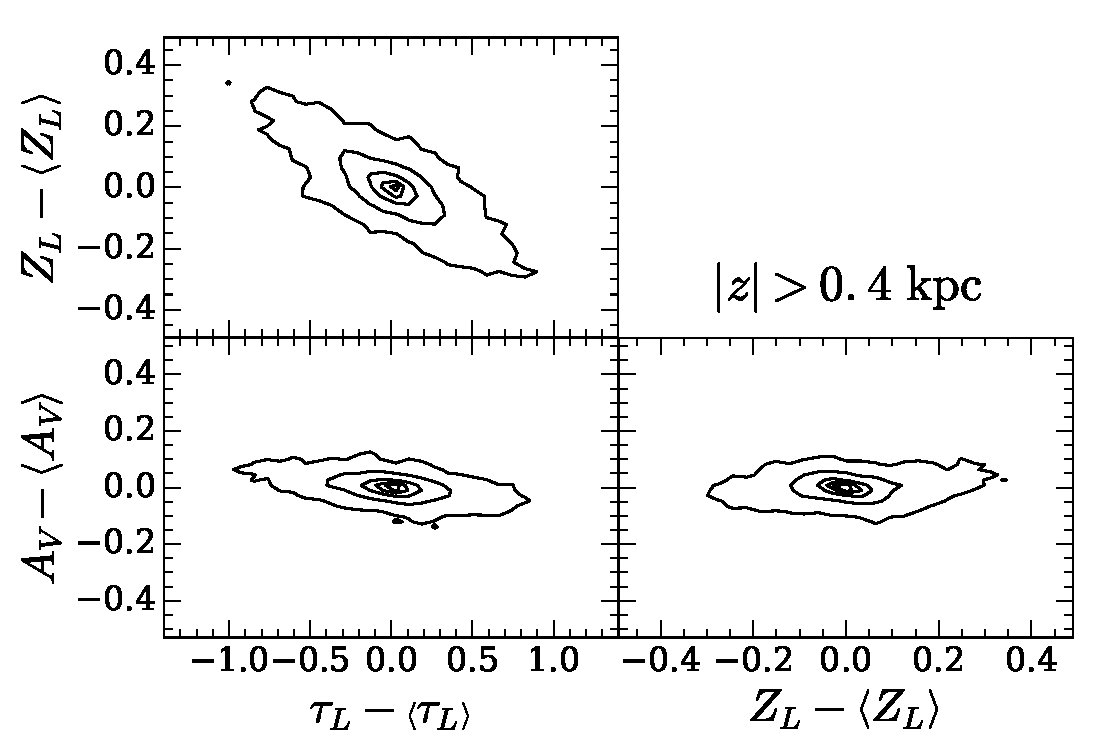
\includegraphics[width=0.48\textwidth]{891_2/figs/MC_covarcont_above.pdf}
  \caption[Covariance between uncertainties in $\tau_L$, $Z_L$, and
    $A_V$]{\fixspacing\label{891_2:fig:MC_covar}Dervied parameters for
    all iterations of the Monte Carlo noise perturbations for all
    apertures. To remove real differences in values between apertures
    the values for each aperture are zeroed to the mean of the 100
    noise perturbations. \emph{left:} Data for apertures below
    \val{0.4}{kpc}. \emph{right:} Data for apertures above
    \val{0.4}{kpc}. The countour levels are 0.5\%, 10\%, 40\%, 70\%,
    and 90\%.{\bf ADE: Maybe loose 0.5\% level?} }
\end{figure*}

Stochastic uncertainty in ($\tau_L$, $Z_L$, $A_V$) that arises during
full spectral fitting is driven by two effects: uncertainty in the
true shape of our galaxy SED and degeneracies between age, extinction,
and metallicity. The uncertainty of the SED of NGC 891 is already
quantified, it is exactly the error spectrum computed as part of the
data reduction described in \ref{chap:891_1} and accounts for
uncertainty in wavelength calibration, sky subtraction, and flux
calibration.

%+++++++++++++++++
%% {\bf MAB: above par. may be a bit redundant with intro par. for the
%%   section, but I would keep the intro par. as is and modify here
%%   accordingly. Pay attention to your use of the term ``shape of the
%%   galaxy data.'' I think you might mean the ``shape of the spectral
%%   energy distribution'' but it is important to be clear if you mean
%%   low or high frequency. I think low frequency is relevant in terms of
%%   flux calibration errors and couples most directly to uncertainties
%%   in age and extinction. The higher-frequency errors associated with
%%   shot noise or sky-subtraction are more likely to impact age and
%%   metallicity.  It might be useful to make these distinctions and
%%   discuss here. Also you should note if flux-cal uncertainties have or
%%   have not been included in the analysis, and if not, why not, or why
%%   we don't care.}

Degeneracies in fit parameters are generally well understood, but more
difficult to quantify. The primary degeneracy in our fits is the well
known age/metallicity degeneracy \citep[see, for
  example,][]{Oconnel76,Aaronson78,Worthey94,dePaz02}, whereby a mix
of younger, more metal-rich populations can be spectrally
indistinguishable from a mix of older, more metal-poor
populations. This correlation is especially relevant to our work given
our attempt to simultaneously fit SSPs with multiple metallicities and
ages.

Secondary degeneracies exist between extinction and both age and
metallicity, the amplitudes of which are dependent on the overall age
of the model spectrum. In models with a high fraction of young SSPs
extinction is strongly correlated with age. This is due to the fact
that the stars that make up these populations are so hot that any
metals present will be fully ionized and therefore won't appreciably
contribute to the total opacity. Thus the only way to change the slope
of the continuum is through wavelength dependent attenuation (i.e.,
classical reddening, $A_V$). 

%% Furthermore, in the absence of extinction
%% older populations are redder due to cooler temperatures and increased
%% line blanketing, but younger populations can be extincted to match,
%% over large wavelength ranges, the general continuum shape of old
%% populations. For single populations this effect is minimal; absorption
%% lines can differentiate different population ages independent of
%% continuum shape, but in composite galaxy spectra made from the
%% superposition of many SSPs (i.e., our spectral fits) the amount of
%% light coming from old populations can be decreased (although not
%% eliminated) be increasing the extinction.

In intermediate-aged populations metal absorption lines make up a key
component of the opacity in stellar atmospheres and a higher
concentration of metals absorption lines will ``redden'' the spectrum
through increased line-blanketing at bluer wavelengths in the stellar
photospheres. In this regime there is a strong negative correlation
between metallicity and extinction because the model spectrum can be
reddened by increasing the strengh of these metal lines. The left
panel of Figure \ref{891_2:fig:MC_covar} shows this effect in the ($A_V$,
$Z_L$) plane. As we will see in \S\ref{891_2:sec:SFH}, below \val{0.4}{kpc}
most of the measured light comes from intermediate populations where
the correlation between $A_V$ and $Z_L$ is strongest.

There is a limit to this effect, however; the very oldest SSPs are
cool enough that there is significant metal-line reddening regardless
of the overal metallicity (at least within the range of metallicities
considered here) and increasing the total metallicity will not
appreciably change the shape of the continuum. This effect can be seen
in the right panel of Figure \ref{891_2:fig:MC_covar}; there is very little
correlation between $Z_L$ and $A_V$ in regions dominated by the Old
DFK bin.

%% A secondary degeneracy exists between metallicity and extinction. A
%% pristine spectrum can be reddened either through the presense of
%% wavelength dependent attenuation (i.e., classical reddening) or
%% through the addition of strong metal absorprion lines. Importantly,
%% there is an age dependence to this effect; young populations are so
%% hot that any metals present will be fully ionized and therefore won't
%% contribute to the total opacity so the slope of the continuum is only
%% weakly dependent on metallicity. In intermediate-aged and old
%% populations, on the other hand, metal absorption lines make up a key
%% component of the opacity in stellar atmospheres and a higher
%% concentration of metals will ``redden'' the spectrum by removing
%% black-body continuum from strong absorption features blueward of
%% \val{\asim 5000}{\AA} (e.g., Fe, Mg, G-band, Ca). %Figure here?

%++++++++++++++++++++++++
%% {\bf MAB: You have everything right here, but the paragraph needs some
%%   re-arrangement. I would lead by saying that age and Z both play off
%%   $A_V$, but the relative importance depends on age. I.e., at young
%%   ages (probably $<$ 0.5-1 Gyr) age reigns supreme in wagging $A_V$
%%   and vice versa. For older ages, it's Z vs $A_V$. I think this will
%%   set the stage for your covariance plots latter. ``through the
%%   addition of strong metal absorprion lines'' should become ``through
%%   increased line-blanketing in stellar photospheres at bluer
%%   wavelengths due to strengthened metal absorption lines.'' You
%%   actually say this latter. Like I said, the words are there! I
%%   wouldn't call out the strong lines in terms of the line-blanketing
%%   effect, but rather the forest of weak lines that supreses the real
%%   continuum to a redder pseudo-continuum level. I think Conroy shows
%%   this pseudo-continuum concept in his review, to which you could
%%   refer.}

%% Finally, there can be degeneracies between age and extinction. In the
%% absence of extinction older populations are redder due to cooler
%% temperatures and increased metal absorption, but younger populations
%% can be extincted to match, over large wavelength ranges, the general
%% continuum shape of old populations. For single populations this effect
%% is minimal; absorption lines can differentiate different population
%% ages independent of continuum shape, but in composite galaxy spectra
%% made from the superposition of many SSPs (i.e., our spectral fits) the
%% amount of light coming from old populations can be decreased (although
%% not eliminated) be increasing the extinction.

%++++++++++++++++++
%% {\bf MAB: I think you can wrap this paragraph into the previous one
%%   along the lines noted. Also, since we've mentioned that there is an
%%   age-Z degeneracy, it is probably worth stating that the coarse age
%%   differentiation for when $A_V$ is degenerate with age vs when it is
%%   more degenerate with $Z$ is sufficiently large that the age-$Z$
%%   degeneracy is no significant in altering the discussion.}

To quantify uncertainties caused by these effects we construct a set
of 100 Monte Carlo iterations of each galaxy spectrum. For each
iteration the galaxy flux at a specific wavelength, $f(\lambda)$, is
perturbed by an amount randomly chosen from a normally distributed set
of values with a width equal to the error spectrum computed during
data reduction. Thus, the $k$th Monte Carlo spectrum is $f_k'(\lambda)
= f(\lambda) + r(e(\lambda))$, where $r(\sigma)$ represents a normal
distribution with width $\sigma$ and $e(\lambda)$ is the galaxy error
spectrum. Each of the $f_k'(\lambda)$ spectra are then fit with the
identical method and SSP library (\S\ref{891_2:sec:final_SSP}). The ``true''
value of the fit parameters is then taken to be the mean over all 100
iterations while the total fit uncertainty (i.e., stochastic plus
degeneracies) is defined by an ellipse in ($\tau_L$,$Z_L$,$A_V$) space
that contains 68\% of all Monte Carlo iterations (i.e., a 68\%
phase-space confidence interval). The reported uncertainties for each
individual parameter are the projection of the limits of this ellipse
onto the specific parameter.

The decision to perform Monte Carlo perturbations on our data rather
than the best fit model is similar to the approach taken by PIPE3D
\citep{Sanchez16}, and we feel it yields important
information. Namely, it allows us to quantify how any systematic
differences between our data and the models couple with random
uncertainties in the data. In other words, it fully encapsulates all
sources of uncertainty that affect the final fits.

%+++++++++++++++++
%% {\bf MAB: You want to say something about the approach of using the
%%   data instead of the models for the MC here. (a) This requires you
%%   smooth the data and models (say how much); but (b) it allows you to
%%   determine how any systematics differences between data and models
%%   couples to random errors in the data -- somthing that can't be done
%%   from doing MCs of the models. And just so we aren't attacked by the
%%   Spanish Armada....I think there is a reference to Sanchez who does
%%   the same. We must reference if so.}

Figure \ref{891_2:fig:MC_covar} shows the result of the Monte Carlo runs. In
the majority of apertures our quantities of interest show the expected
degeneracies discussed above (negative age/metallicity correlation,
negative age/extinction correlation, and negative
metallicity/extinction correlation) however there are large group of
apertures that exhibit a \emph{positive} correlation between age and
metallicity (i.e., increasing the metallicity leads to fits that have
older ages). This seemingly backward trend is reasonable (and
expected) in the context of how the reddening affects different aged
populations. Apertures with a positive age/metallicity relation are
concentrated below the age break at \val{0.4}{kpc}
\citepalias{Eigenbrot16a} and thus have a high fraction of total flux
contributed by young SSPs. As discussed above young SSPs have a
continuum shape that is only weakly dependent on metallicity, so
reddening is achieved by increasing $A_V$. Thus, as the fraction of
Young SSPs increases more extinction is needed to match the data. This
increase in total extinction (for a given aperture) then requires the
I2 and Old SSPs to have lower metallicities to counteract the
extinction-induced reddening. This decreases the total metallicity,
$Z_L$, because (as shown in \S\ref{891_2:sec:SFH}) I2 and Old SSPs dominate
the light fraction at all points in the galaxy. Thus, the positive
age/metallicity correlation at small heights is the result of the fact
that metallicity is a weighted average that is mostly dominated by
older SSPs, and that a single extinction value, $A_V$, is applied to
all SSPs in a particular fit.

%% {\bf MAB: I am not sure I buy your conclusion, so I recommend we redo
%%   this starting with the parts we do agree on, and then get to the
%%   more challenging bits. So start with a first-order description of
%%   Fig \ref{891_2:fig:MC_covar}, as follows:

%% $\bullet$ $A_V$-age: negative at all heights; stronger at lower $z$

%% $\bullet$ $A_V$-Z: negative at hi-$z$; flat at low-$z$.

%% $\bullet$ Z-age: more weakly correlated at low $z$, with a hint that
%%   it is a postive correlation; strongly negative correlation at
%%   hi-$z$.  Concerning the hint, see comment in figure caption. This is
%%   likely more than a hint but you need to discuss significance of
%%   contour levels.

%% Then I would turn first to discuss the r.h. panels for $z>0.4$ kpc for
%% the older pops and describe how it makes sense. The big deal is
%% age-metallicity; well known. But note there is a little degeneracy in
%% AV and age, although apparently none between AV and Z which refutes
%% our line-blanketing spit-balling earlier in the text.

%% Then I would turn to the less-intuitive situation at low heights where
%% ages are lower. (You should either or both hark back to Paper I to
%% quote what you think are the characteristic ages in the $z<$0.4 kpc
%% and $z>0.4$ kpc bins, or compute the average from later sections in
%% the paper.  Note in text or caption.)

%% Here's what I don't buy (yet):

%% ``...young SSPs have a continuum shape that is only weakly dependent
%% on metallicity, so reddening is achieved by increasing $A_V$. This
%% increase in total extinction (for a given aperture) requires older
%% SSPs to have lower metallicities to counteract the extinction-induced
%% reddening. Thus, the positive age/metallicity correlation at small
%% heights is the result of the fact that metallicity is a weighted
%% average that is mostly dominated by older SSPs, and that a single
%% extinction value, $A_V$, is applied to all SSPs in a particular fit.''

%% The underlying premise is this:

%% ``metallicity is a weighted average that is mostly dominated by older
%% SSPs''

%% But it is not correct. The metallicity is light-weighted, so if the
%% population is young $Z_L$ is a measure of the metallicity of the young
%% stars. 

%% Here's my theory:

%% ``because young SSPs have a continuum shape that is only weakly
%% dependent on metallicity, variations in the stellar population age and
%% $A_V$ both serve to be the primary ways to redden the continuum shape.
%% Consequently these model parameters are strongly negatively
%% correlated.  When increases in model age overly serve to fit the
%% reddened continuum, to compensate for the increased metal line
%% strength one might expect the model metallicy to diminish. In fact the
%% opposite is seen, i.e. surprisingly age and metallicity are {\it
%%   positively} correlated. We believe this is an artifact of having
%% adopted a constant extinction value for all age templates. A more
%% realistic model would tend to apply more extinction to the younger
%% populations. As a consequence, when the ratio of young to old stars is
%% over-estimated, this diminishes the model metal-line equivalent
%% widths, and to compensate the model metallicity must increase.''

%% If this is what you mean, then it is just that your wording is
%% confusing or unclear.

%% }  
 
\begin{figure*}
  \centering
  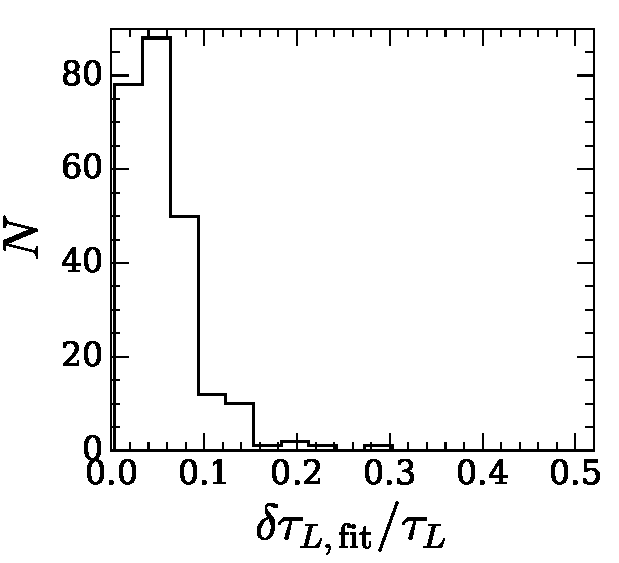
\includegraphics[width=0.31\textwidth]{891_2/figs/fit_uncertainty_MLWA.pdf}
  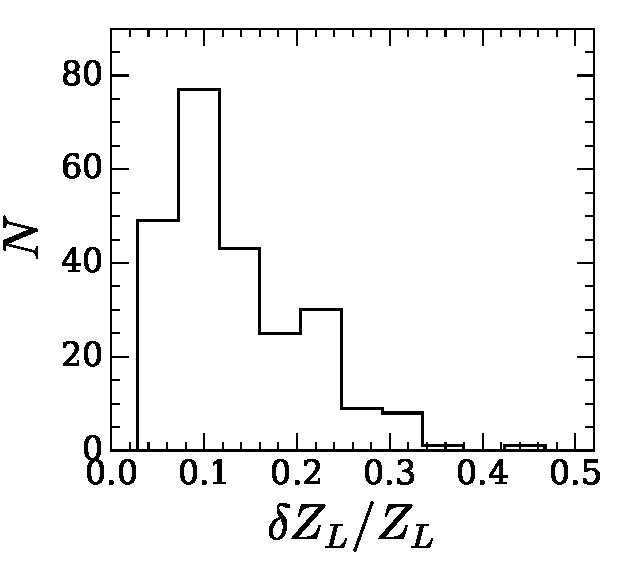
\includegraphics[width=0.31\textwidth]{891_2/figs/fit_uncertainty_MLWZ.pdf}
  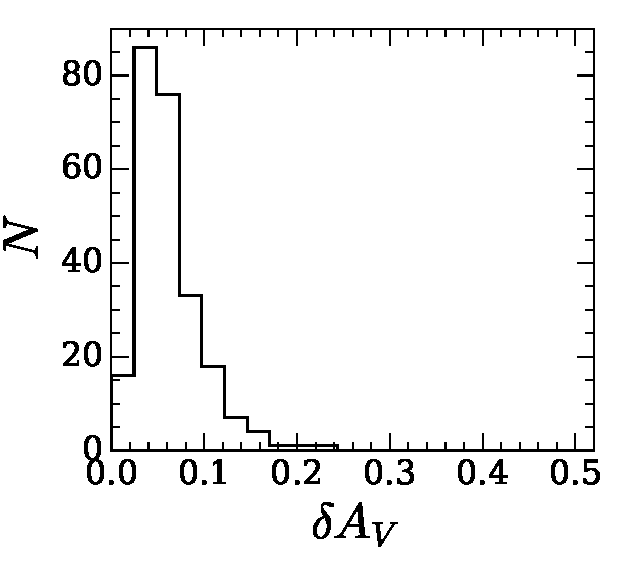
\includegraphics[width=0.31\textwidth]{891_2/figs/fit_uncertainty_TAUV.pdf}
  \caption[Distributions of fit uncertainties in $\tau_L$, $Z_L$,
    $A_V$]{\fixspacing\label{891_2:fig:fit_err_hist}Distribution of
    parameter uncertainties in age, metallicity, and extinction
    derived from full spectral fitting.  The uncertainties are 68\%
    confidence limits on all three parameters simultaneusly based on
    the Monte Carlo perturbations described above.}
\end{figure*}

The fact that a purely random perturbation of our data results in fits
that clearly show the expected astrophysical degneracies indicates
that these degeneracies are primary source of fitting uncertainty. In
other words, uncertainty in our SSP fits is driven mainly by
similarities between different model SSPs; uncertainty in the shape of
our galaxy spectra are only a secondary source of fitting uncertainty.

%% {\bf MAB: The hard question then is why did we bin to such high
%% S/N?}  

%% ADE comment: The binning was based on theory. Here is the
%% reality. Better to be in this case than a situation where data
%% uncertainty drives our total uncertainty.

We compute total fitting uncertainty using the method described above
separately for each aperture. The values thus derived constitute all
sources uncertainty that arise from the simultaneous measurement of
the three parameters. Figure \ref{891_2:fig:fit_err_hist} shows the
distribution of uncertainties in age, metallicity, and
extinction. Fitting uncertainties are on the order of 5\% for most
apertures, but the distribution of uncertainty in metallicity is
broader than either $\tau_L$ or $A_V$ and can reach \asim 30\% in the
worst cases.

%+++++++++++++++
%% {\bf MAB: You want to emphasize that ``total'' here includes the
%%   degeneracies, i.e., these are not marginalized, but are the
%%   uncertainties in simultaneous measurement of all three parameters.

%--------------
%% {\bf $>>>$ How do these uncertainties compare to what you predicited in
%%   Paper I?}

\subsection{Systematic Uncertainty in DFK Ages}
\label{891_2:sec:sys_err}

Computing a weighted age for a superposition of model SSPs requires
assigning a specific age to each individual SSP, which, in turn,
requires making an assumption about the star formation history (SFH)
across the range of ages spanned by the SSP age bin (see Table
\ref{891_2:tab:dfk}). Different SFHs have minimal impact on the youngest
SSPs due to their narrow age range, but the oldest SSPs span a range
of over \val{7}{Gyr} and thus the age assigned to this bin can vary by
the same magnitude, depending on the assumed SFH. Because of this, the
choice of SFH creates systematic uncertainty in the computed value of
$\tau_L$. This uncertainty is primarily a consequence of the fact that
old stellar spectra are essentially constant over a large age
range. In other words, these old populations do not provide enough
information in their spectral shape to yield precisely defined ages.

%+++++++++++++++++
%% {\bf MAB: Here I think it is worth reminding the reader that this
%%   problem of the older DFK bins isn't due to a bad choice on our or
%%   M15's part, but rather that the width of the bins reflects our
%%   ignorance, or rather, where we do not have information.}

To quantify this systematic uncertainty we compute $\tau_L$ as derived
from 100 Monte Carlo SFHs. For each Monte Carlo iteration we assign
each DFK bin an age that is randomly selected from a uniform
distribution bounded by the limits of the age bin given in Table
\ref{891_2:tab:dfk}. These ages correspond to $t_i$ in Equation
\ref{891_2:eq:MLWA}, which allows us to compute a different $\tau_L$ for
each iteration. It is important to note that $t_i$ is the only
quantity that changes between iterations; the specific SSP weights
($W_{L,i,j}$) are held constant at their best fit values. The standard
deviation of $\tau_L$ across all 100 Monte Carlo iterations quantifies
the systematic uncertainty that results from assuming a SFH.

By chosing $t_i$ completely randomly from within the corresponding age
bin we allow completely unconstrained SFHs, which makes our computed
uncertainty an upper limit. The drawback of this approach is an
almost-certain over estimation of the true systematic uncertainty, but
the benefit is that we are not required to make assumptions about the
general form of the SFH. In this way, our computation
captures not only our lack of knowledge about the specific shape of
SFH, but also our lack of knowledge about the general form of SFH
(e.g., bursty versus smooth).

\begin{figure}
  \centering
  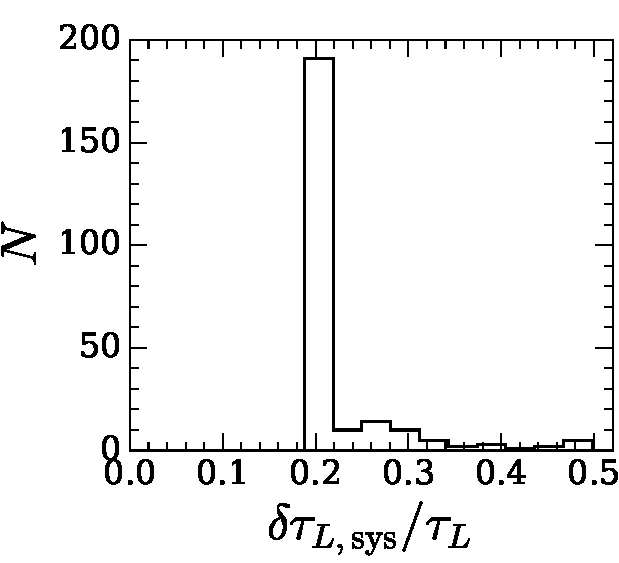
\includegraphics[width=0.45\textwidth]{891_2/figs/sys_uncertainty_hist.pdf}
  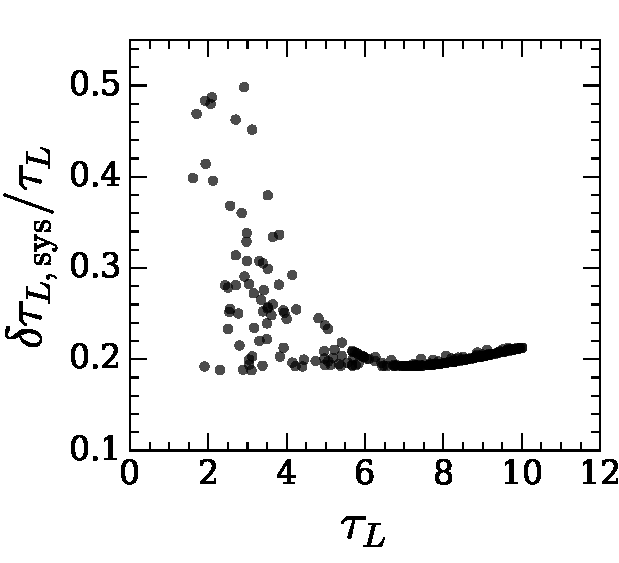
\includegraphics[width=0.45\textwidth]{891_2/figs/sys_uncertainty.pdf}
  \caption[Distribution of systematic uncertainties in
    $\tau_L$]{\fixspacing\label{891_2:fig:sys_err}\emph{top:}
    Distribution of systematic uncertainty that arises from assuming a
    star formation history. The uncertainties are the standard
    deviation of 100 values derived from a random assignment of ages
    to the SSP basis set. \emph{bottom:} The same systematic
    uncertainties as a function of $\tau_L$.}
\end{figure}

The top panel Figure \ref{891_2:fig:sys_err} shows the distribution of
systematic uncertainties in $\tau_L$. In the majority of our apertures
this uncertainty is \asim 20\%, but there is a tail with high
fractional uncertainties that extends up to 50\%, which, as shown in
the bottom panel, comes from apertures with $\tau_L < \val{\asim
  5}{Gyr}$. As we will see in \S\ref{891_2:sec:SFH} I2 and O populations
make up the largest contributions to the total light in all apertures,
even those with a significant fraction of younger populations and it
is these older populations that have the largest systematic
uncertainty due the large range of ages they represent. Thus in all
apertures the systematic uncertainty is dominated by the presence of
old populations. Figure \ref{891_2:fig:MLWA_sys_err} shows these
uncertainties in the context of the age gradients presented in
\S\ref{891_2:sec:rz}; given the magnitude of these uncertainties it is
difficult to make strong statements on the detailed structure and
trends in age or any other measured quantity.

%++++++++++++++
%% {\bf MAB: Spell out the computation for me. You have 100 sets
%% of DFK ages. For each aperture you take the best fit DFK weights,
%% compute 100 values of $\tau_L$, and then take the mean
%% and standard deviation of these values. That ratio is plotted in the figure.}

\begin{figure}
  \centering
  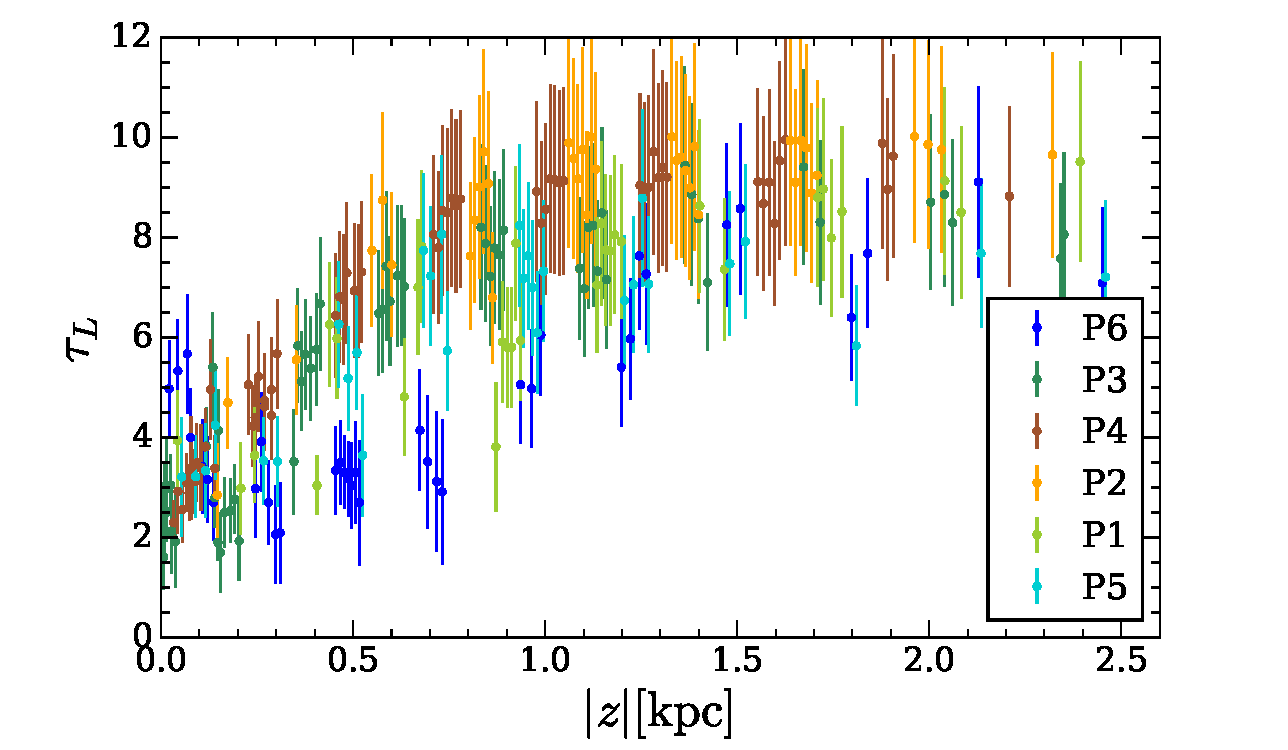
\includegraphics[width=\columnwidth]{891_2/figs/MLWA_sys_err.pdf}
  \caption[Systematic $\tau_L$ uncertaities in relation to our data]
          {\fixspacing\label{891_2:fig:MLWA_sys_err}$\tau_L$ as a
            function of height above the midplane showing the
            magnitude of the systematic uncertainties that arise from
            assuming a star formation history.}
\end{figure}

Despite this bleak picture, we urge the reader to take solace in the
fact that the systematic uncertainties presented above are an extreme
upper limit and ignore NGC 891 as a coherent galaxy. In other words,
it is unreasonable to assume that the SFH within NGC 891 varies on
time scales greater than a dynamical timescale (\val{\asim
  1}{Gyr}). Thus, when assesing trends in $\tau_L$, $Z_L$, or $A_V$ we
can say with confidence that points near each other in phase space
likely come from the same underlying population(s), despite the large
systematic uncertainties. It is only on large physical and time scales
that these uncertainties become relevant. Furthermore, in
\S\ref{891_2:sec:SFH} we find evidence that the general form of SFH is
mostly invarient over the portion of NGC 891 we measure. For these
reasons we choose not to include systematic uncertainties in the final
results shown in \S\ref{891_2:sec:results}, where we draw conclusions about
the detailed, small-scale structure of NGC 891. If we were to compare
the global results for NGC 891 presented here to other galaxies with
potentially different SFH then the systematic uncertainties would be
relevant.

%------------------
%% {\bf MAB: I agree with everything you say here, but I would word it
%%   differently, emphasizing earlier that Figure \ref{891_2:fig:sys_err} is
%%   the worst case of the worst case.}

%% ADE comment. Not sure what you mean here, I think it does a good
%% job as it is.
